\section{Trabajo realizado durante trabajo terminal 1} \label{TrabajoTerminal1}

En esta sección se habla a manera de resumen el trabajo realizado durante el 
periodo correspondiente a trabajo terminal 1. La división de esta sección 
queda organizada en dos subsecciónes: una para la etapa de preprodución y 
otra para los dos primeros \textit{sprints} de la estapa de produción. 

\subsection{Presentado en TT1}\label{tt1}
A continuación se muestra lo presentado en TT1, que representa la investigación, análisis y prototipos del proyecto.

\subsubsection{Contexto}\label{contexto}
Primero nos encontramos a determinar que es la cultura; aquella que define la identidad de un individuo por sus creencias religiosas, de pensamiento, sentimentales y sociales. Mientras que la historia son todos los sucesos pasados dentro de un espacio específico. Entonces la cultura histórica es aquellos aspectos arquitectónicos, de pensamiento, éticas y morales, grupos de pertenencia y convivencia. Dentro de la hultura histórica encontramos que el 41\% de los mexicanos no asisten a eventos culturales y presentan una gran desinformación de ella.

Luego nos encontramos que existen formas de presentar cualquier tema o actividad dentro de los juegos. A partir de eso investigamos sobre los videojuegos, juegos que se presentan a través de un medio visiual o auditivo en el que existe interacción por diferentes dispositivos de entrada. Dentro de los videojuegos hay clasificaciones por contenido, que son las utilizadas para determinar el tipo de público al que va dirigido, además de que es una clasificación conveniente para limitar compra y venta. Sin embargo existen muchas más clasificaciones, en donde el tipo de contenido, dispositivo u objetivo es su pertenencia.

\subsubsection{Viabilidad}\label{viabilidad}
Con esta información ya en mano, buscamos sobre la situación actual de comercio de los videojuegos. Pasando primero por los ingresos a nivel mundial y en que dispositvos en el año 2017; a nivel mundial se tiene un ingreso de \$108.9 mil millones de dolares, el 42\% está en los dispositvos móviles, tanto teléfonos inteligentes como tabletas, el resto queda en la computadora y consolas. Así México queda en el doceavo lugar de consumo de videojuegos a nivel mundial, con un ingreso percibido de \$1.4 mil millones de dolares en una población de 130 millones de mexicanos. De la población en México el 20\% juega videojuegos, de ese porcentaje 45\% juega en el celular y 40\% juega de una a dos veces por semana.

\subsubsection{Análisis}\label{analisis}
Una vez contemplada la información, se decide que el proyecto se haga en un dispositvo móvil android, dado que el 86\% de los usuarios de dispositivos móviles tienen android y como versión mínima 5.0 lolipop con su uso de 32\% de las personas.

La metodología a usar será Hundle, que consiste en un parecido a la metología scrum solo que está adaptada a la creación y desarrollo de videojuegos, donde se establece un proceso general de preproducción,  producción y postmortem. Destacando aquí que se hicieron algunos ajustes dentro de la parte de preproducción agregando y modificando apartados daddo que eran necesarios aclarar antes de empezar con el proyecto.

Luego se pasó a definir las herramientas de desarrollo, donde se escogió debido a su flexibilidad multiplataforma el motor de juego Unity y como herramientas de dibujo corel draw x5 y photoshop.

Como arquitectura a usar se eligió modelo vista controlador, donde se dividirá el código en controladores, actores y auxiliares, estos últimos ayudarán a los controladores y actores en situaciones específicas donde no se encuentre en ninguna de estas características.

\subsubsection{Progresión y prototipos}\label{proypro}
Ya realizadas las investigaciones y análisis previo para el proyecto, se estableció la progresión que iba a tener el juego, junto con definir las interfaces que contendría y su interacción entre ellas.
Se estableció la mecánica del juego donde se definía los botones de acción del personaje, el espacio de características del personaje y un apartado para determinar otros factores como items o vida del enemigo.

Ya en los prototipos se pasó a el maquetado de los niveles uno y dos, determinando personajes y eventos, así como prototipos de uso de la herramienta Unity.Al final dando como resultado dos prototipos conteniendo el nivel uno y dos y un prototipo de uso de la herramienta.

\subsection{Etapa de Preproducción}\label{EtapaPreproduccion}
Esta etapa corresponde a la planeación analisis y diseño del juego. Como lo indica 
la metodología \textit{Huddle}, para esta etapa se trabaja en el desarrollo del 
documento de diseño del juego. Esta etapa queda del desarrollo queda dividida en 
cuatro \textit{sprints}.

\subsubsection{Primer Sprint Huddle de Preproducción}\label{Prepro01}
Antes de iniciar el diseño del juego se realiza un trabajo de investigación 
sobre la cultura azteca. Esta investigación abarca:
\begin{itemize}
        \item \textbf{La sociedad mexica:} su historia tradiciones y clases sociales. 
        \item \textbf{Mitología mexica:} Dioses, mito de los cinco soles, mito de la 
        creación del hombre del maíz, el Mictlán.
        \item \textbf{Historia de la Malinche:} Historia del personaje antes y después 
        de la llegada de los españoles.
\end{itemize} 
 
Durante la etapa de investigación se selecciona la información histórica que 
sera relevante y útil para la narrativa del juego y el diseño de su jugabilidad. 
Para la investigación histórica de esta etapa se consultan libros, códices, 
páginas de Internet, artículos de investigación e incluso se visitan museos 
como el templo mayor.

\subsubsection{Segundo Sprint Huddle de Preproducción}\label{PrePro02}
En este \textit{sprint} se redactan las primeras secciones del documento de diseño del 
juego \textit{Yolotl}. Se inicia con la idea concepto y con el tema del juego. De igual 
forma se selecciona un nombre para el juego a desarrollar: \textit{Yolotl}. 
Para algunos juegos la mecánica es la primera es ser definida; no obstante, 
por la naturaleza del juego como herramienta de transmisión de cultura, 
\textit{Yolotl} nace con su historia. La historia de \textit{Yolotl} pasa por 
diferentes etapas de diseño; siendo modificada gradualmente, pero manteniendo 
algunos elementos clave como la lucha contra la divinidad. 
\\
\par
En la etapa del concepto también se define la plataforma para la que será 
el juego: dispositivos móviles con sistema operativo Android 5.2. Por su parte 
se decide utilizar un motor de juego como herramienta de desarrollo, pues esto 
permite centrarse en el diseño e implementación de aquellos elementos que 
diferencien a \textit{Yolotl} del resto de juegos, tal como su mecánica, sus 
personajes, etc. Luego de investigar sobre los motores de juegos disponibles, 
se elije Unity 3D como ambiente de desarrollo.
\\
\par
Una vez teniendo la idea concepto se define la visión del juego y sus mecánicas. 
En cuestión de las mecánicas el enfoque por el que se opta es el de mantener 
el juego con mecánicas simples y familiares para aquellos jugadores que ya habían 
tenido alguna experiencia con algún juego de plataformas, sin descartar algunos 
detalles que le dieran identidad al juego en cuanto a su jugabilidad. Paralelamente 
a la preproducción, se inicia el desarrollo de un primer demo con el fin de 
familiarizarse con la herramienta de Unity3D, este demo incluye las mecánicas más 
simples del juego.
\\
\par
Con la historia, la visión y la mecánica definidas se procede a puntualizar los 
estados del juego, diseñar las interfaces gráficas de navegación y de interacción 
con el personaje. Para ver la versión final de las interfaces se puede consultar 
anexo \ref{Anexo:Intefaces}.

\subsubsection{Tercer Sprint Huddle de Preproducción}
En el tercer Sprint se definen la cantidad de niveles y en que consiste
cada uno, de igual forma se establecen los objetivos de cada nivel, la recompensa 
a obtener una vez completado el mismo, los enemigos a vencer y las cinemáticas que 
fungen como transiciones entre niveles.  
\\
\par
Al mismo tiempo que se diseñan los niveles, se detallan los 
personajes tanto a nivel narrativo como a nivel de jugabilidad, definiendo habilidades 
para los enemigos, los niveles en los que parecerían y sus acciones dentro de 
la historia. Para esta parte se trata de obtener la mayor fidelidad posible a 
los mitos y códices. En el anexo \ref{Anexo:Personajes} se habla a mayor detalle 
sobre el diseño de los personajes.

\subsubsection{Cuarto Sprint Huddle de Preproducción} 
En el cuarto sprint se termina de escribir el argumento del juego, de esta 
destapa se obtiene el guión literario del juego. En este \textit{sprint} también se definen 
elementos de ambientación para el juego tales como la música de fondo, los 
efectos de sonido y los efectos especiales. 
\\
\par
De igual forma, en este \textit{sprint} se especifican las armas de los personajes, los 
ítems; quedando diseñados tanto a nivel de comportamiento como a nivel 
visual. Al igual que con los personajes se busca que las armas, tanto en 
comportamiento como en diseño, se mantengan lo más fiel posible a los mitos 
y leyendas de donde se basaron.
\\
\par
Con el cuarto \textit{sprint} se finaliza la etapa de preproducción, obteniendo así un 
documento de diseño lo suficientemente detallado como para iniciar el diseño 
del juego a nivel de ingeniera. 

\subsection{Etapa de producción}
En esta sección se habla del trabajo realizado durante los dos primeros 
\textit{sprints} de esta etapa, ya que fueron desarrollados durante los meses 
correspondientes al trabajo terminal 1. Todos los \textit{sprints} del la etapa 
de producción posteriores al segundo \textit{sprint} son abordados en la sección 
\ref{TrabajoTT2}.

\subsubsection{Primer Sprint Huddle de Producción.}
En este \textit{sprint} se realiza un análisis del documento de diseño, en consecuencia 
de este análisis se se diseña el videojuego en materia de las clases que lo 
componen y el modelo bajo el que funcionaría el juego a nivel de programación. 
\\
\par
Haciendo uso del paradigma orientado a objetos se propone emplear tres tipos 
de clases:
\begin{itemize}
        \item \textbf{Actores:} Son las clases que modelan a los enemigos, los ítems, 
        los coleccionables, los checkpoints y al jugador.
        \item \textbf{Controladores:} Son las clases encargadas de gestionar la partida 
        y la navegación entre interfaces. Estas clases desencadenan eventos conforme a 
        las acciones de las clases actoras. Estas clases también son las encargadas de 
        verificar que se cumplan las reglas de los niveles.
        \item \textbf{Auxiliares:} Estas clases ayudan al funcionamiento de los actores 
        y los controladores. Estas clases también se encargan le vincular datos con 
        las clases controladoras como efectos de sonido, música, datos para la 
        progresión entre niveles.
\end{itemize}
El modelo planteado permite reutilizar parte del demo generado durante la etapa 
de preproducción. Por lo aque en este \textit{sprint} se inicia la integración 
del código del primer demo con el comportamiento modelado por las clases definidas 
en el párrafo anterior. 
\\
\par
En el primer \textit{sprint} de Producción también se crean los \textit{sprites} del 
primer nivel utilizando la herramienta de modelado en \textit{3D Blender}. En la
figura \ref{fig:Modelos3D} se pueden observar algunos de los modelos creados. Al 
finalizar este \textit{sprint} se determina la no viabilidad del modelado en 3D de los 
\textit{sprites} por cuestiones de tiempos; en consecuencia, se descarta este 
método para generar los \textit{sprites} y se inicia el desarrollo de los 
\textit{sprites} a partir de otras técnicas de animación más tradicionales.

\begin{figure}[h]
  		\centering
   		\subfigure[Modelo de \textit{Malinalli} generado en \textit{Blender}.] {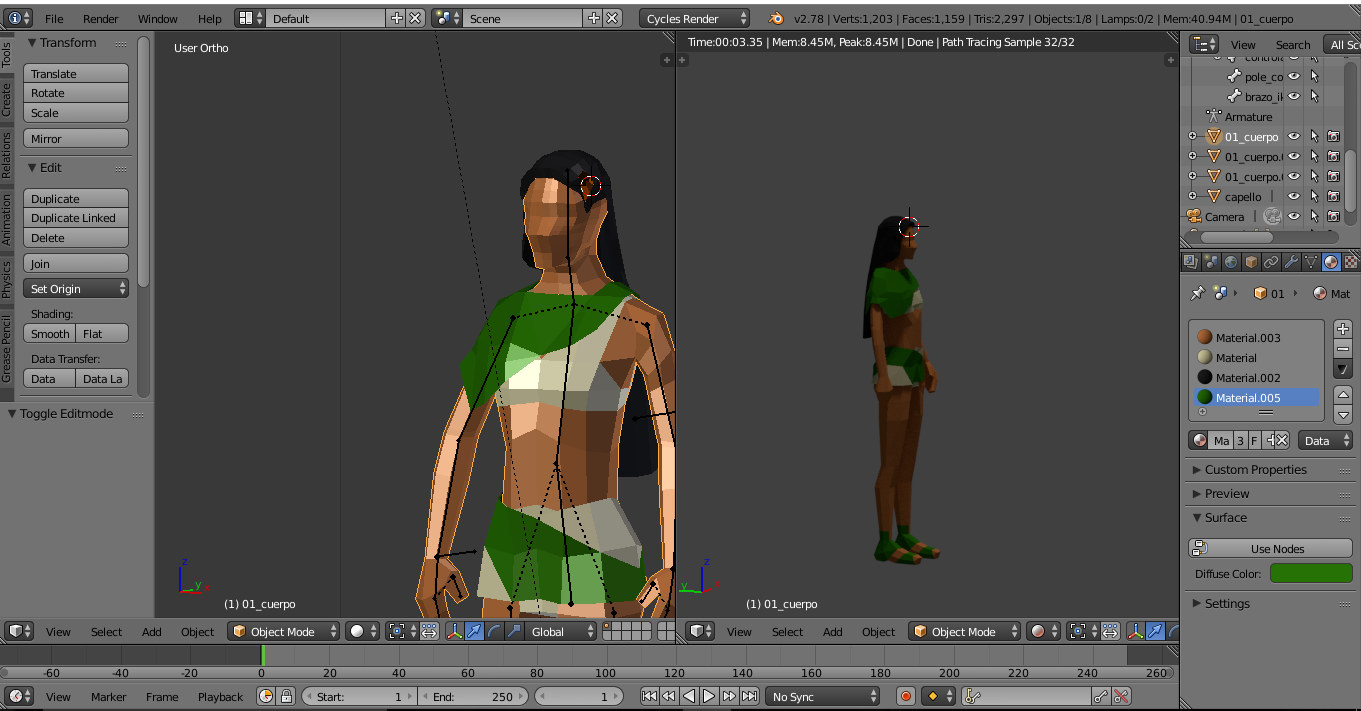
\includegraphics[width=0.3 \textwidth]{02Antecedentes/Imagenes/Malinalli_proceso.png}}
   
 		\subfigure[Modelo de \textit{Xólotl} generado en \textit{Blender}.]{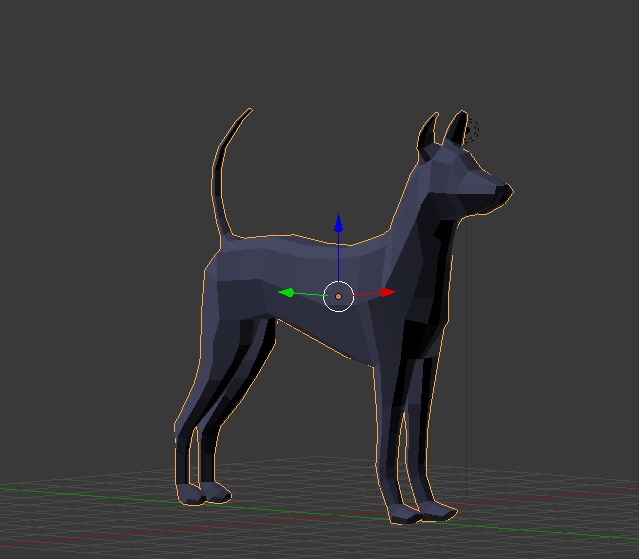
\includegraphics[width=0.3 \textwidth]{02Antecedentes/Imagenes/xolo.jpg}}
 	
		\subfigure[Modelo de un templo generado en \textit{Blender}.] {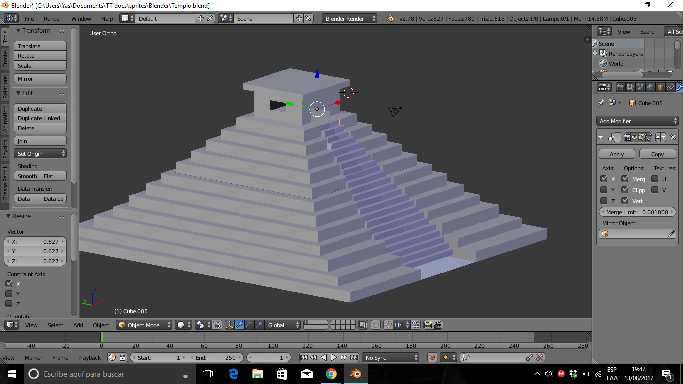
\includegraphics[width=0.3 \textwidth]{02Antecedentes/Imagenes/templo.png}}
		
		\subfigure[Modelo de una mujer comerciante generado en \textit{Blender}.] {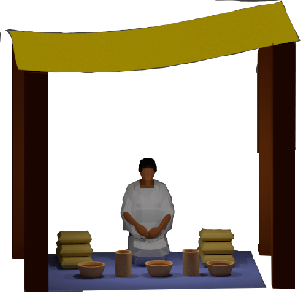
\includegraphics[width=0.3 \textwidth]{02Antecedentes/Imagenes/Mujer04_game.png}}
		
  		\caption{Modelos de personajes y objetos crados en \textit{Blender} (Autoria propia).}
  		\label{fig:Modelos3D}
\end{figure}

\subsubsection{Segundo Sprint Huddle de Producción.}
En este \textit{sprint} se inicia el desarrollo de los \textit{sprites} 
con \textit{Adobe Photoshop} y \textit{Corel Draw}. A la par se inicia la 
maquetación de la etapa de selva del nivel uno. En este sprint se logran 
terminar todos los \textit{sprites} referentes al primer nivel del juego 
tales como: 

\begin{itemize}
        \item Objetos de fondo: Arbustos, árboles, jarrones y cajas. 
        \item Imagen de fondo: Fondo de la selva, la ciudad y el menú principal. 
        \item Ciudadanos del mercado: Comerciantes, nobles y esclavos. 
        \item \textit{Xólotl} en su forma \textit{xoloitzcuintle}: Bloques de 
        animacion para correr y normal.
        \item \textit{Malinalli} sin la caracola: Bloques de animación correr, 
        saltar y normal.
\end{itemize}
Una vez terminados los \textit{sprites} referentes al nivel uno estos se integran 
al código permitiendo tener un segundo prototipo con la siguiente funcionalidad:
\begin{itemize}
        \item Control de personaje por medio de la GUI.
        \item Transiciones entre interfaces.
        \item Personaje seguible que aparece en el primer nivel funcional.
        \item Funcionamiento básico del controlador de diálogos.
\end{itemize}

%\subsection{Presentado en TT1}\label{tt1}
A continuación se muestra lo presentado en TT1, que representa la investigación, análisis y prototipos del proyecto.

\subsubsection{Contexto}\label{contexto}
Primero nos encontramos a determinar que es la cultura; aquella que define la identidad de un individuo por sus creencias religiosas, de pensamiento, sentimentales y sociales. Mientras que la historia son todos los sucesos pasados dentro de un espacio específico. Entonces la cultura histórica es aquellos aspectos arquitectónicos, de pensamiento, éticas y morales, grupos de pertenencia y convivencia. Dentro de la hultura histórica encontramos que el 41\% de los mexicanos no asisten a eventos culturales y presentan una gran desinformación de ella.

Luego nos encontramos que existen formas de presentar cualquier tema o actividad dentro de los juegos. A partir de eso investigamos sobre los videojuegos, juegos que se presentan a través de un medio visiual o auditivo en el que existe interacción por diferentes dispositivos de entrada. Dentro de los videojuegos hay clasificaciones por contenido, que son las utilizadas para determinar el tipo de público al que va dirigido, además de que es una clasificación conveniente para limitar compra y venta. Sin embargo existen muchas más clasificaciones, en donde el tipo de contenido, dispositivo u objetivo es su pertenencia.

\subsubsection{Viabilidad}\label{viabilidad}
Con esta información ya en mano, buscamos sobre la situación actual de comercio de los videojuegos. Pasando primero por los ingresos a nivel mundial y en que dispositvos en el año 2017; a nivel mundial se tiene un ingreso de \$108.9 mil millones de dolares, el 42\% está en los dispositvos móviles, tanto teléfonos inteligentes como tabletas, el resto queda en la computadora y consolas. Así México queda en el doceavo lugar de consumo de videojuegos a nivel mundial, con un ingreso percibido de \$1.4 mil millones de dolares en una población de 130 millones de mexicanos. De la población en México el 20\% juega videojuegos, de ese porcentaje 45\% juega en el celular y 40\% juega de una a dos veces por semana.

\subsubsection{Análisis}\label{analisis}
Una vez contemplada la información, se decide que el proyecto se haga en un dispositvo móvil android, dado que el 86\% de los usuarios de dispositivos móviles tienen android y como versión mínima 5.0 lolipop con su uso de 32\% de las personas.

La metodología a usar será Hundle, que consiste en un parecido a la metología scrum solo que está adaptada a la creación y desarrollo de videojuegos, donde se establece un proceso general de preproducción,  producción y postmortem. Destacando aquí que se hicieron algunos ajustes dentro de la parte de preproducción agregando y modificando apartados daddo que eran necesarios aclarar antes de empezar con el proyecto.

Luego se pasó a definir las herramientas de desarrollo, donde se escogió debido a su flexibilidad multiplataforma el motor de juego Unity y como herramientas de dibujo corel draw x5 y photoshop.

Como arquitectura a usar se eligió modelo vista controlador, donde se dividirá el código en controladores, actores y auxiliares, estos últimos ayudarán a los controladores y actores en situaciones específicas donde no se encuentre en ninguna de estas características.

\subsubsection{Progresión y prototipos}\label{proypro}
Ya realizadas las investigaciones y análisis previo para el proyecto, se estableció la progresión que iba a tener el juego, junto con definir las interfaces que contendría y su interacción entre ellas.
Se estableció la mecánica del juego donde se definía los botones de acción del personaje, el espacio de características del personaje y un apartado para determinar otros factores como items o vida del enemigo.

Ya en los prototipos se pasó a el maquetado de los niveles uno y dos, determinando personajes y eventos, así como prototipos de uso de la herramienta Unity.Al final dando como resultado dos prototipos conteniendo el nivel uno y dos y un prototipo de uso de la herramienta.